%%%%%%%%%%%%%%%%%%%%%%%%%%%%%%%%%%%%%%%%%%%%%%%%%%%%%%%%%%%%%%%%%%%%%%%%
%    INSTITUTE OF PHYSICS PUBLISHING                                   %
%                                                                      %
%   `Preparing an article for publication in an Institute of Physics   %
%    Publishing journal using LaTeX'                                   %
%                                                                      %
%    LaTeX source code `ioplau2e.tex' used to generate `author         %
%    guidelines', the documentation explaining and demonstrating use   %
%    of the Institute of Physics Publishing LaTeX preprint files       %
%    `iopart.cls, iopart12.clo and iopart10.clo'.                      %
%                                                                      %
%    `ioplau2e.tex' itself uses LaTeX with `iopart.cls'                %
%                                                                      %
%%%%%%%%%%%%%%%%%%%%%%%%%%%%%%%%%%
%
%
% First we have a character check
%
% ! exclamation mark    " double quote  
% # hash                ` opening quote (grave)
% & ampersand           ' closing quote (acute)
% $ dollar              % percent       
% ( open parenthesis    ) close paren.  
% - hyphen              = equals sign
% | vertical bar        ~ tilde         
% @ at sign             _ underscore
% { open curly brace    } close curly   
% [ open square         ] close square bracket
% + plus sign           ; semi-colon    
% * asterisk            : colon
% < open angle bracket  > close angle   
% , comma               . full stop
% ? question mark       / forward slash 
% \ backslash           ^ circumflex
%
% ABCDEFGHIJKLMNOPQRSTUVWXYZ 
% abcdefghijklmnopqrstuvwxyz 
% 1234567890
%
%%%%%%%%%%%%%%%%%%%%%%%%%%%%%%%%%%%%%%%%%%%%%%%%%%%%%%%%%%%%%%%%%%%
%

%AIP Reprint Class%%%%%%%%%%%%%%%%%%%%%%%%%%%%%%%%%%%%%%%%%%%%%%%%%%%%%%%%%%%%%%%%%%%%%%%%%%%%%
\documentclass[aps,prl,amsmath,amssymb,reprint,superscriptaddress]{revtex4-1} %preprint version
\usepackage{graphicx}% Include figure files
\usepackage{dcolumn}% Align table columns on decimal point
\usepackage{bm}% bold math
\usepackage{epstopdf}

    \renewcommand{\topfraction}{0.9}    % max fraction of floats at top
    \renewcommand{\bottomfraction}{0.8}    % max fraction of floats at bottom
    \setcounter{topnumber}{2}
    \setcounter{bottomnumber}{2}
    \setcounter{totalnumber}{4}     % 2 may work better
    \setcounter{dbltopnumber}{2}    % for 2-column pages
    \renewcommand{\dbltopfraction}{0.9}    % fit big float above 2-col. text
    \renewcommand{\textfraction}{0.07}    % allow minimal text w. figs
    \renewcommand{\floatpagefraction}{0.7}    % require fuller float pages
    \renewcommand{\dblfloatpagefraction}{0.7}    % require fuller float pages
    \setlength{\abovecaptionskip}{5pt}
    \setlength{\belowcaptionskip}{5pt}
    \setlength{\parskip}{0pt}
    \setlength{\textfloatsep}{5pt} 

%%%%%%%%%%%%%%%%%%%%%%%%%%%%%%%%%%%%%%%%%%%%%%%%%%%%%%%%%%%%%%%%%%%%%%%%%%%%%%%%%%%%%%%%%%%%%%%%%%

%IOP preprint class %%%%%%%%%%%%%%%%%%%%%%%%%%%%%%%%%%%%%%%%%%%%%%%%%%%%%%%%%%%%%%%%%%%%%%%%%%%%%%
%\documentclass[12pt]{iopart}
%\newcommand{\gguide}{{\it Preparing graphics for IOP journals}}
%Uncomment next line if AMS fonts required
%\usepackage{iopams}
%\usepackage{graphicx}
%\usepackage{epstopdf}  
%%%%%%%%%%%%%%%%%%%%%%%%%%%%%%%%%%%%%%%%%%%%%%%%%%%%%%%%%%%%%%%%%%%%%%%%%%%%%%%%%%%%%%%%%%%%%%%%%%
%Slava's inserts %%%%%%%%%%%%%%%%%%%%%%%%%%%%%%%%%%%%%%%%%%%%%%%%%%%%%%%%%%%%%%%%%%%%%%%%%%%%%%
%\usepackage{amsfonts}
%\usepackage{amssymb}

%\newcommand{\ptt}[1]{\frac{\partial#1}{\partial t}}
%\newcommand{\vvec}{\mathbf{v}}
%\newcommand{\Bvec}{\mathbf{B}}
%\newcommand{\Evec}{\mathbf{E}}
%\newcommand{\Jvec}{\mathbf{J}}
%\newcommand{\Avec}{\mathbf{A}}
%%%%%%%%%%%%%%%%%%%%%%%%%%%%%%%%%%%%%%%%%%%%%%%%%%%%%%%%%%%%%%%%%%%%%%%%%%%%%%%%%%%%%%%%%%%%%%%%%%

\begin{document}
\title{Spatial magnetic correlation functions and Taylor microscale in a turbulent MHD laboratory plasma}

\author{A. Wan}
\affiliation{Swarthmore College, Swarthmore, PA, USA}
\author{D.A. Schaffner}
\affiliation{Swarthmore College, Swarthmore, PA, USA}
\author{V.S. Lukin}
\affiliation{Space Science Division, Naval Research Laboratory, Washington, DC, USA}
\author{W.H. Matthaeus}
\affiliation{Bartol Research Institute and Department of Physics and Astronomy, University of Deleware, Newark, DE, USA}
\author{M.R. Brown}
\affiliation{Swarthmore College, Swarthmore, PA, USA}
\date{\today}
\begin{abstract}
Spatial correlation analysis is used to determine the Taylor microscale and magnetic Reynolds number in a turbulent, high beta ($\beta \sim 0.1$), high flow ($M \sim 0.4$), laboratory MHD plasma.  An unambiguous measure of the magnetic Reynolds number is estimated from the Taylor microscale and the correlation length, then compared to a calculation using the Spitzer resistivity.
\end{abstract}

\maketitle

\section{Introduction}

Two point velocity correlation functions have been measured in conventional fluids for decades~\cite{frisch95,Belmabrouk98}, but two point magnetic spatial correlations in plasmas are less common.  The first proper two-point single time measurements of the magnetic correlation function in the solar wind plasma were performed by Matthaeus, et al \cite{Matthaeus05}.  They used simultaneous magnetic field data from several spacecraft, including the four Cluster spacecraft flying in tetrahedral formation.  Simultaneous measurements were performed with separations ranging from $150~km$ (using pairs of Cluster satellites) to $350~R_E$ ($2.2 \times 10^6~km$).  From measurements of the outer correlation length, and the Taylor microscale, they report an effective magnetic Reynolds number of the solar wind $R_{mT}  = 230,000$.

In a set of follow-up papers, Weygand, et al \cite{Weygand07,Weygand09,Weygand10,Weygand11} have modified and improved the earlier result.  In particular, they describe a method using fits of Cluster separations \cite{Weygand07} from 100 to $10^6~km$, and extrapolating the Taylor microscale down to zero separation.  We discuss this method below.  These more detailed measurements confirm the earlier work  \cite{Matthaeus05} and find a solar wind magnetic Reynolds number of $R_{mT}  = 260,000 \pm 20,000$.  In addition, using data in the magnetospheric plasma sheet (tailward of Earth), they find a much smaller Reynolds number $R_{mT}  = 111 \pm 12$ since the outer correlation length is much smaller in the plasma sheet.  Anisotropies in the correlation function parallel and perpendicular to the local magnetic field were studied in separate papers \cite{Weygand09,Weygand10}, with longer correlation lengths measured parallel to the local field.  Variations with solar wind speed were also studied \cite{Weygand11}.

This paper presents the first measurements of spatial correlation function in a high beta ($\beta \sim 0.1$), high Mach ($M \sim 0.4$) turbulent laboratory plasma in the wind-tunnel configuration of the Swarthmore Spheromak Experiment. The Taylor microscale and Taylor Reynolds number of this turbulent plasma are computed directly from spatial correlation functions. The value for the magnetic Reynolds number, $R_{mT}$, based on the Taylor microscale, compares well to the value of $R_{m}$ calculated using an estimation of the Spitzer resistivity from electron temperature measurements.  The benefit of the Taylor Reynolds number is that it can be measured without measuring the flow speed, or the microscopic diffusivity (based on Spitzer resistivity, for example).  

%These values can be compared to similar quantities found in space plasma observations or {\it in-situ} measurements from satellites. An example of the advantage of laboratory experiment in such turbulent research is given through a comparison of the spatial correlation functions in single plume versus colliding plume plasmas. The results indicate that colliding or merging plasma have a slightly smaller Taylor microscale than single plume or non-merging plasmas.

\section{Theory and Techniques}

A useful measure of fully developed turbulence is the spatial correlation function.  For a magnetohydrodynamic (MHD) plasma, the radial correlation function of the magnetic field can be written
%
\begin{equation}
\mathcal{R}(r) =  \langle {\bf b(x) \cdot b(x + r)} \rangle
\label{eq:correlation1}
\end{equation}
%
where {\bf b} is the fluctuating part of a turbulent magnetic field (${\bf B}(x, t) = {\bf B_0 + b}$) and $ \langle*** \rangle$ represents an ensemble average of several realizations.  The correlation function is normalized by $\mathcal{R}(0) =  \langle {\bf b(x) \cdot b(x)} \rangle$.  For well-behaved turbulence, the magnetic fluctuations at two points should become uncorrelated at large spatial separation and the correlation function should vanish ($\mathcal{R} \rightarrow 0$ as $r \rightarrow \infty$).  

The magnetic Taylor microscale, $\lambda_{T}$, can be formally defined as
%
\begin{equation}
\lambda_T^2 \equiv \frac{\langle {\bf b}^2 \rangle}{\langle (\nabla \times {\bf b})^2 \rangle}.
\label{eq:tayscale}
\end{equation}
%
This definition identifies the Taylor microscale as the scale associated with mean square spatial derivatives of the fluctuating magnetic field $\bf{b}$, i.e. the thickness of a typical current layer. A similar definition of the Taylor microscale in conventional fluids involves spatial derivatives of the fluctuating velocity field~\cite{frisch95}. It is at this scale that one would expect dissipation effects to become important, although actual dissipation likely occurs at smaller, kinetic scales~\cite{Matthaeus08} ($k_D \lambda_T = R_m^{1/4}$, where $R_m$ is the magnetic Reynolds number defined below).  We expect that the Taylor microscale should be on the order of but larger than the Larmor scale ($\rho_i \approx 1~mm$ in the SSX wind tunnel) and the ion inertial scale ($c/\omega_{pi} \approx 6~mm$ in SSX). For small values of $r$, the correlation function can be approximated as
%
\begin{equation}
\mathcal{R}(r) \approx  1 - \frac{r^2}{2 \lambda_T^2} 
\label{eq:correlation2} 
\end{equation}
%
The Taylor microscale is extracted by fitting a parabolic function of the form in Equation~\ref{eq:correlation2} to our measured spatial correlation functions. By separately fitting a parabola to the spatial correlations for different numbers of points, a plot of Taylor microscale as a function of number of fit points is constructed. This curve is then extrapolated to determine the Taylor microscale at zero separation, a procedure called Richardson extrapolation. 

Finally, a Taylor Reynolds number can be written~\cite{frisch95}
%
\begin{equation}
R_{mT}  = \left(\frac{\lambda_{C}}{\lambda_T} \right)^2 
\label{eq:RM-eff}
\end{equation}
%
where, $\lambda_{C}$, is the correlation length. This length, $\lambda_{C}$, is less formally defined but represents the scale at which fluctuations become de-correlated.  It is also one measure of the largest scale in the turbulence, or an outer scale.  Often, the integral scale, defined as
%
\begin{equation}
\lambda_{I}  = \int_0^\infty \mathcal{R}(r) dr
\label{eq:tayscale2}
\end{equation}
%
can be used, but can be problematic when the measured $\mathcal{R}(r)$ does not approach zero. 

In this paper, we adopt two extremes for the correlation length.  First, the shortest correlation length uses the integral scale definition above, but only after fitting the measured $\mathcal{R}(r)$ to a Gaussian function and using this fit function in Equation~\ref{eq:tayscale2}.  A longer correlation length comes from a direct measurement of the energy containing scale of the relaxing magnetic structure.  In a previous paper \cite{Gray13} we found the wavenumber of the large scale twisted structure was $k a = 1.292$.  Since the radius of the wind tunnel is $a = 7.8~cm$, we find $\lambda_{L} =38~cm$.  

From these values of the correlation length, estimates of the Taylor Reynolds number are made using Equation~\ref{eq:RM-eff}. These can be compared to a computation of the magnetic Reynolds number derived by evaluation of the Spitzer conductivity, $\sigma_{SP}$,
\begin{equation}
R_m = \mu_0 V \sigma_{SP} L.
\label{eq:RM-calc} 
\end{equation}
%
where $\sigma_{SP}\sim T_{e}^{-3/2}$. Using a measured value of $T_e = 10~eV$ for the SSX wind tunnel \cite{Zhang11}, and $V=20~km/s$, the Spitzer magnetic Reynolds number is 577. The outer scale, L, is taken as the energy-containing scale $\lambda_{L} = 38~cm$.  Note that this determination of $R_m$ requires knowledge of the microscopic dissipation (Spitzer resistivity) and flow speed.

\section{Experimental Apparatus}

\begin{figure}[!htbp]
\centerline{
\includegraphics[width=8.5cm]{Images/simulation_diagram_radcorr_paper}}
\caption{\label{fig:chamber} Diagram showing orientation of plasma, plasma gun source, and 16 channel, 3-axis magnetic pick up coil. The probe extends radially into the plasma at the midplane. Blue lines represent simulation generated magnetic field lines of the plasma.}
\end{figure}

The measurements are made on the MHD wind-tunnel configuration of the Swarthmore Spheromak Experiment (SSX). Plasma guns located on both sides of a $0.155~m$ diameter, $0.86~m$ long cylindrical copper tube produce highly magnetized, dense plasma ($B \sim 0.5~T, n \sim 1\times 10^{21}~m^{-3}$) using a plasma gun source. The turbulence is generated as the initial plasma structure (called a spheromak) undergoes a tilt-instability and expands into the copper tube or MHD wind-tunnel. Details of the formation process are discussed in previous work on SSX~\cite{schaffner14a,schaffner14b,brown14,brown15a,brown15b}. Magnetic fluctuations are recorded by a 16-channel, 3-axis probe array of single-loop pickup coils located at the midplane and protruding radially into the cylindrical chamber. The measurement points span a region from about $1~cm$ off the cylindrical axis to the inner edge of the chamber and are spaced by about $4.6~mm$. The coils measure fluctuations in $dB/dt$ using a 14-bit, 65 MHz D-TACQ digitizer and then numerically integrated to construct $B(t)$ timeseries for each loop axis aligned in cylindrical coordinate directions: $B_{r}$, $B_{\theta}$, and $B_{z}$. Data analyzed from each configuration consists of at least forty shots to create an ensemble average. The spatial correlation functions are measured during the stationary phase of the turbulence; a time period of $40$ to $60~\mu s$ after the initial discharge. 

The experimental data is also compared with Hall-MHD simulated versions of the wind-tunnel plasma generated using the HiFi framework~\cite{schaffner14a}. The simulation data consisted of magnetic field measured along 8 equally-spaced radii at the midplane of the simulated flux conserver. The epoch used was $46-56~ \mu s$, chosen to capture fluctuations in the simulations that qualitatively resembled the $40-60\ \mu s$ epoch of the experimental data. Visualization of this simulation-generated data is shown in Figure~\ref{fig:chamber}.

\section{Results}

Figure~\ref{fig:brbtbz} shows the radial correlation functions, $\mathcal{R}(r)$, constructed by computing the cross correlation, $C_{ij} = \langle B_x^i B_x^j\rangle$ of the innermost channel, $i$, with each of the $j=1-16$ spatial channels as a function of spatial distance from that initial channel and normalizing to the value at $\mathcal{R}(0)$. The three spatial directions are shown separately, $B_{r}$, $B_{\theta}$, and $B_{z}$ for Figure~\ref{fig:brbtbz}a,b, and c respectively. Within each subplot, a Gaussian fit using all sixteen points is shown as well as a parabolic fit using Eq.~\ref{eq:correlation2} with the four innermost points. The error bars for each plot indicate the standard deviation of the mean of cross-correlation coefficients over the forty shots. Visible inspection shows that the statistical spread in the radial correlation function increases with separation distance and that the scatter for $B_{z}$ is greater than that for $B_{r}$ and $B_{z}$. This difference may relate to the fact that $B_{z}$ is in the direction of the bulk flow of the plume and may be more affected by fluctuations in flow than the other directions. The innermost point is also offset from the central axis of the cylinder by about 1cm so that extent of the signal reaches all the way to the wall of the chamber where boundary effects may have an effect. In particular, the radial correlation function for $B_{r}$ does not reach as close to zero correlation as the other two directions. This effect may be caused by the presence of stray field lines that are able to leak out of the slot in the cylinder through which the magnetic probe is inserted. These field lines would in general be radially aligned and tend to increase the correlation along the $B_{r}$ direction.

\begin{figure}[!htbp]
\centerline{
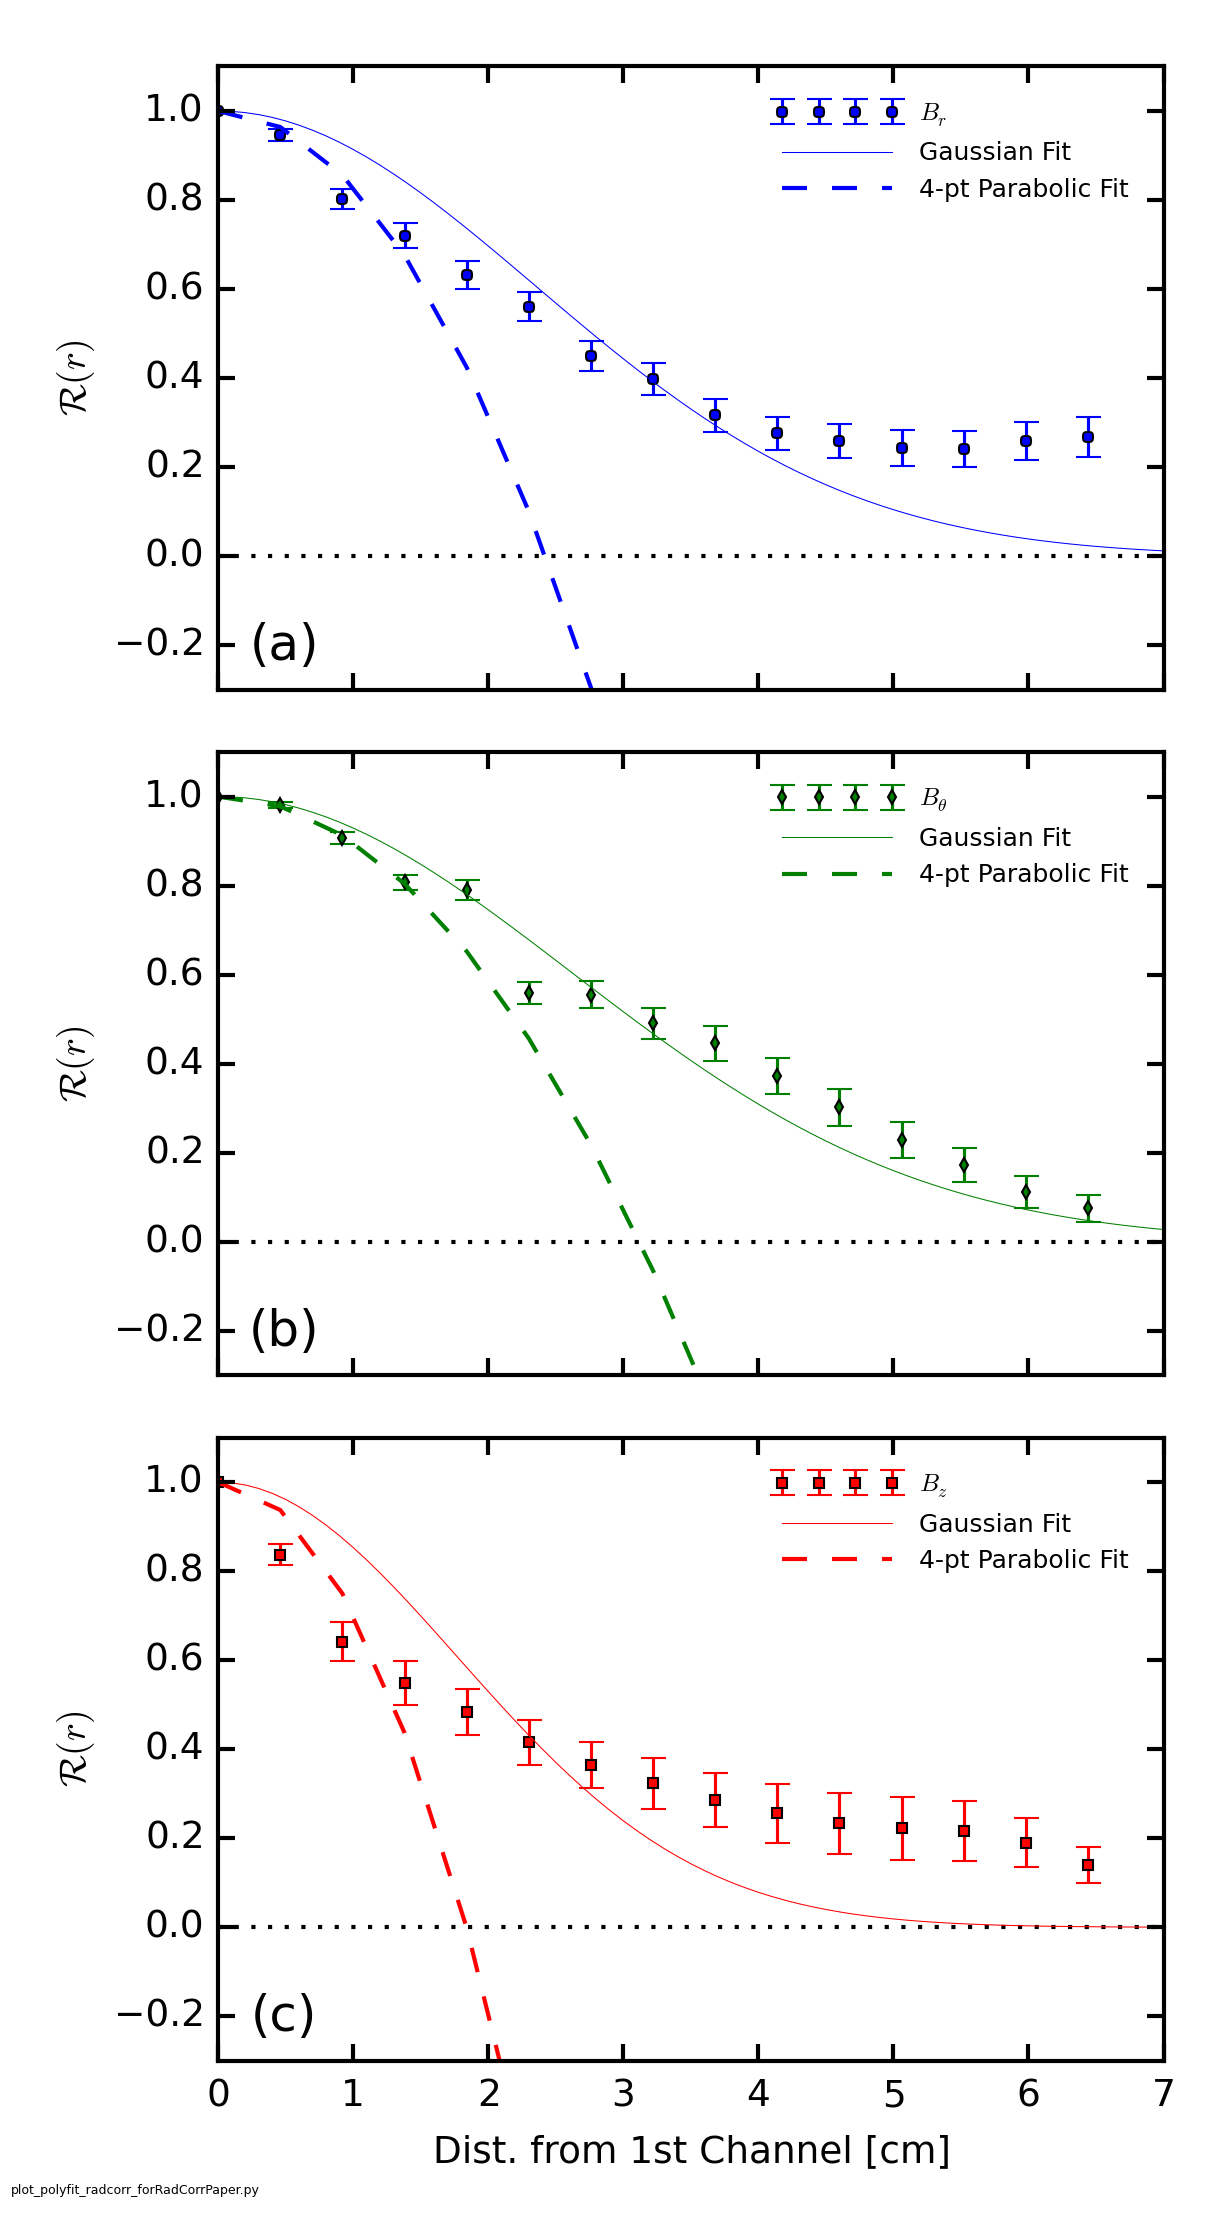
\includegraphics[width=8.5cm]{RadialCorrelation_BrBtBz_1mWb_wdetrend.png}}
\caption{Single plume correlation functions for magnetic field in the (a) $\hat{r}$, (b) $\hat{\theta}$, (c) $\hat{z}$ directions. Error bars indicate the standard deviation of the mean over forty shots. Solid lines are best fit Gaussian functions to the full $\mathcal{R}(r)$ and dashed lines are a representation of the parabolic fits using just the inner four points.}
\label{fig:brbtbz}
\end{figure}

The radial correlation functions from the experiment can be compared to those made from the Hall-MHD simulation. The solid lines in Figure~\ref{fig:comparisons} are the radial correlations from Figure~\ref{fig:brbtbz} plotted on the same axes. The dashed lines represent radial correlation functions computed for the simulated $B_{r}$, $B_{\theta}$, and $B_{z}$. Note that the innermost point in the simulation is closer to the central axis than the experimental data so the radial correlation function spans a larger range in the simulation. The shapes of the correlation functions for the three directions matches well to the simulation. The $B_{z}$ radial correlation function for both experiment and simulation drop faster than the other two directions which again might be an indication of the effect of the bulk flow on the correlation. The $B_{\theta}$ experimental correlation matches well up to about 4cm. The simulation $B_{r}$ and $B_{\theta}$ correlation functions are very similar; this is perhaps unsurprising given that there should generally be no distinction between the two directions since they are both perpendicular to the bulk flow direction. The difference between $B_{r}$ and $B_{\theta}$ then observed in the experiment might be reflecting experimental issues associated with the probe.

\begin{figure}[!htbp]
\centering
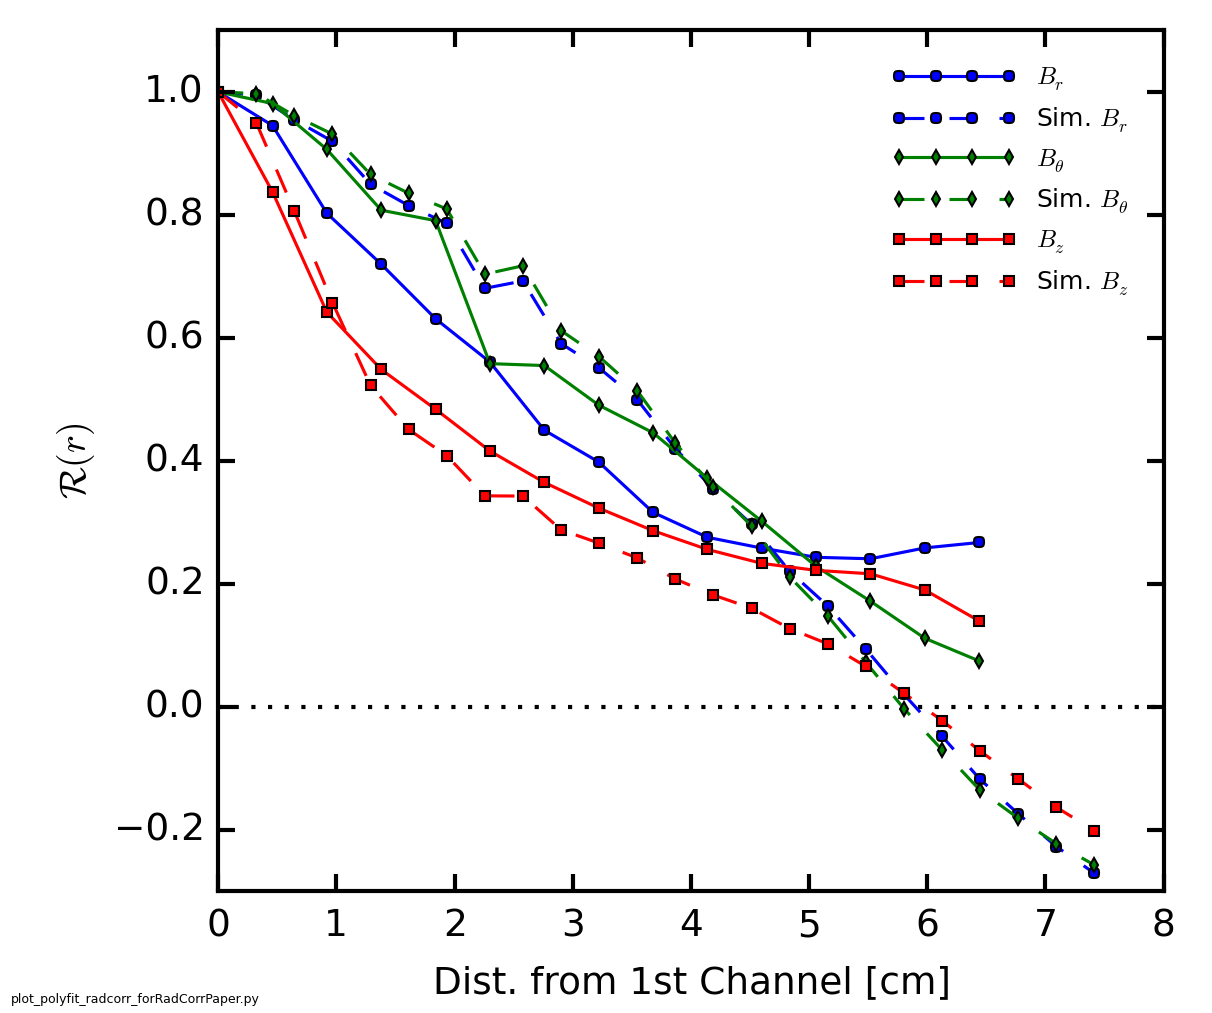
\includegraphics[width=8.5cm]{Exp1mWb_vsSim_wdetrend.png}
\caption{\label{fig:comparisons}Radial correlation functions, $\mathcal{R}(r)$ for the three experimental (solid lines) and simulation (dashed lines) directions: $B_r$-circles, $B_{\theta}$-diamonds, and $B_z$-squares. Note that $B_z$ for both experiment and simulation match well and follow a steeper trend than the other two directions. $B_{\theta}$ experimental matches well to the simulated quantity as well, while $B_r$ falls away from the simulation curve as it approaches the boundary wall.}
\end{figure}

\begin{figure}[!htbp]
\centerline{
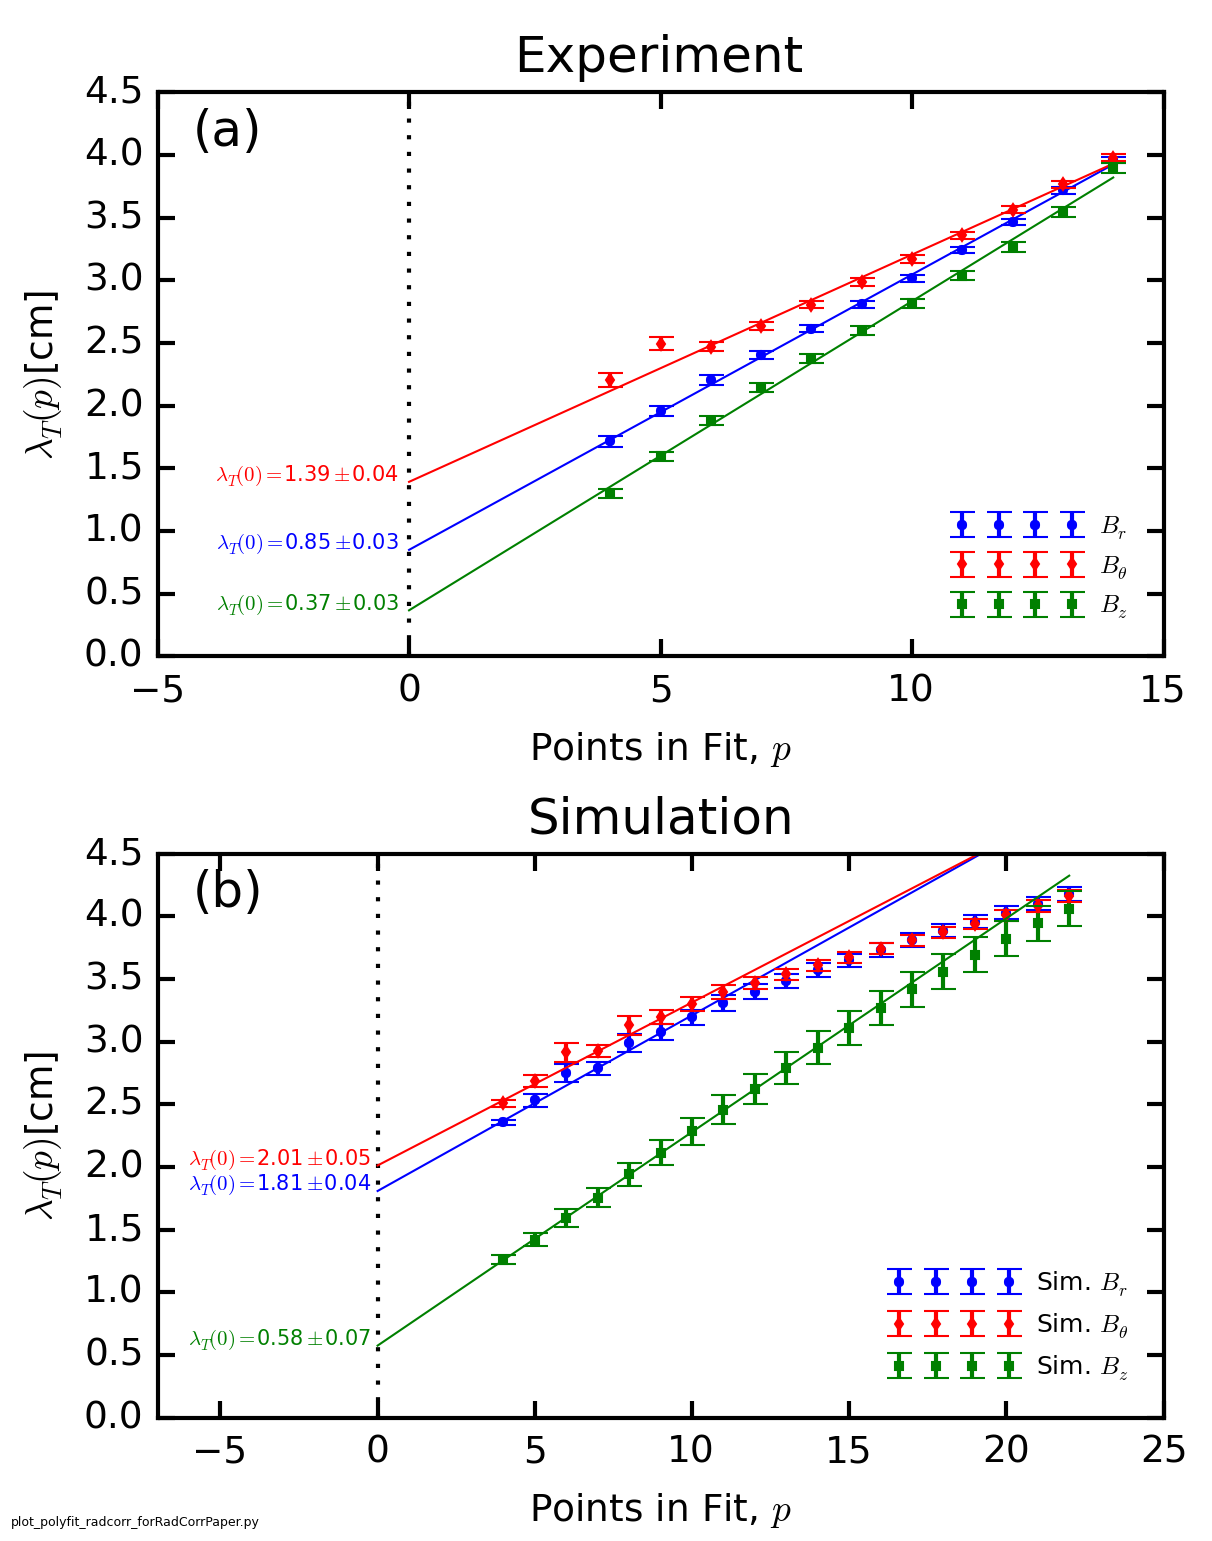
\includegraphics[width=8.5cm]{RichardsonExtrap_BrBtBz_1mWb_wdetrend.png}}
\caption{\label{fig:extrap} Determination of $\lambda_T(0)$ using Richardson extrapolation for (a)Experiment and (b)Simulation. Each point represents the quantity $\lambda_{T}$ computed from the fit of Equation~\ref{eq:correlation2} using the inner $p$ points from $\mathcal{R}(r)$ for the fit.}
\end{figure}

Following a similar procedure as in Weygand 2007~\cite{Weygand07}, the Taylor microscale at zero separation, $\lambda_{T}(0)$, is determined using Richardson extrapolation for both the experimental and simulation data and separately for each of the three orthogonal axes. A parabolic fit using Eq.~\ref{eq:correlation2} using a range of points from the maximum number available---15 for the experiment, 23 for the simulation--down to a four point fit. From these fits, $\lambda_{T}(p)$ is computed where $p$ is the number of points used for the fit. The values for $\lambda_{T}(p)$ are shown in Figure~\ref{fig:extrap} as a function of $p$ for all of the cases and field directions. The error bars reflect the spread in the fit and incorporates the goodness-of-fit as well as the number of points used to make the fit. An extrapolated value of the Taylor microscale is determined by applying a linear fit to the values of $\lambda_{T}(p)$ using the error bars as a relative weight for the fit and extracting the y-intercept of the fit. Note that for the simulation, the linear fit is made using only half of the points closest to the center since there is a clear change in trend, while the experimental data is fit over the entire range.  The values for each fit and error are indicated in both Figure~\ref{fig:extrap} and in Table~\ref{tab:Rms1}.

The Richardson extrapolation procedure shows that the $B_{z}$ fluctuations have the smallest Taylor microscale for both simulation and experiment. This value might be expected to be lower as it incorporates both the decorrelation radially as well as that due to the bulk flow. The simulation values for $\lambda_{T}(0)$ for $B_{r}$ and $B_{\theta}$ are larger than what is observed in experiment. This might imply that additional physics is still needed for the simulation to better reach the experimental values, though the numbers are qualitatively well-matched. In addition, the computed values for the Taylor microscale are consistent with dissipation scale lengths determined through previously reported spectral analysis on this same dataset~\cite{schaffner14c}. In this work, the breakpoint in the spectrum was shown to be consistent with the ion inertial scale which for this plasma is about 0.6cm. Since Taylor microscale theory suggest that $\lambda_{T}(0)$ should be the largest dissipation scale observed, the values computed here are all near, but larger the ion inertial scale length, again with the exception of the experimental $B_{z}$.

The magnetic Reynolds number, $R_{m}$ can be estimated using the value of the $\lambda_{T}(0)$ and an outer scale, $\lambda_{C}$, as in Equation~\ref{eq:RM-eff}. As discussed, this outer scale can be defined in a number of ways; thus, a maximum and minimum value are presented. The minimum value of $\lambda_{C}$ used is the integral scale, $\lambda_{I}$ computed from Equation~\ref{eq:tayscale2} using the best fit Gaussian of $\mathcal{R}(r)$ rather than the radial correlation function itself since neither the experimental or simulation $\mathcal{R}(r)$ is shown at large enough $r$ to converge. The values for $\lambda_{I}$ are shown in the second column of Table~\ref{tab:Rms1}. The largest possible outer scale is taken from the helical structure of the final state of the plasma, $\lambda_{L}$ = 38cm. It should be noted that this is a maximum scale since it was determined in the fully relaxed state of the plasma evolution. It is likely that the outer scale during the plasma evolution is smaller.

The computed values for $R_{mT}$ are shown in columns three and four of Table~\ref{tab:Rms1}. Though all three directions are reported for both experimental and simulated data, focus should be on the value of $B_{\theta}$ since this quantity is least affected by either the flow of the plasma itself as $B_{z}$ appears to be, or possible probe effects as $B_{r}$ appears to be. The experimental value for magnetic Reynolds number for $B_{\theta}$ using the maximum outer scale is $R_{mT} = 744\pm38$ while the simulated value is $R_{mt} = 356\pm17$. On the other hand, the value of $R_{m}$ estimated using Spitzer resistivity is,
\begin{equation}
R_{m} = \mu_0 V \sigma_{SP} \lambda_L = 577.
\label{eq:spitzer} 
\end{equation}
Both experimental and simulated values are on the right order of magnitude and end up being about $30\%$-exp/$40\%$-sim off from the estimated value.

\begin{table} [htbp]
\caption{\label{tab:Rms1}Comparison of Taylor Microscale and Taylor magnetic Reynolds numbers for various cases.}
\begin{tabular}{lcccc}
\toprule
Dataset								& $\lambda_{T}$[cm]	&$\lambda_{I}$[cm]	&$R_{mT}(\lambda_{I})$&$R_{mT}(\lambda_L)$\\
\hline		  					
Exp.\\
\hline
$B_{r}$ 							& 0.85$\pm$0.03 		&	2.95							& 12.03$\pm$0.91 			& 1998$\pm$152\\
$B_{t}$			 					& 1.39$\pm$0.04 		&	3.27							& 5.52$\pm$0.28 			& 744$\pm$38\\
$B_{z}$ 							& 0.37$\pm$0.03 		&	2.22							& 36.57$\pm$6.67			& 10683$\pm$1953\\
\hline
Sim.\\
\hline
$B_{r}$			 					& 1.81$\pm$0.04 		&	3.35							& 3.43$\pm$0.16 			& 441$\pm$21\\
$B_{t}$ 							& 2.01$\pm$0.05 		&	3.37							& 2.80$\pm$0.13 			& 356$\pm$17\\
$B_{z}$ 							& 0.56$\pm$0.07 		&	2.05							& 12.65$\pm$2.88 			& 4359$\pm$992\\
\end{tabular}
\end{table}

This paper demonstrates the ability to calculate the magnetic Reynolds number of an experimental system using only a radial correlation function and without needing to determine electron temperature or flow speed. Taylor microscale values at zero-separation were determined using the radial correlation function and the Richardson extrapolation method. The resulting scales were consistent with prior measurements of the dissipation scale. Comparison of experimental data with a Hall-MHD simulation shows that the simulation qualitatively captures the same relative amount of magnetic turbulence as the experiment based on an evaluation of the magnetic Reynolds number. Comparisons between experiment and simulation also indicate where experimental issues regarding probe and chamber boundaries may arise. Also, direction of the measurement with respect to bulk flow direction also appears to significantly affect the correlation of the fluctuation signals. Computation of magnetic Reynolds number based on measurement of the Taylor microscale are also qualitatively in agreement with computation using Spitzer resistivity. The method for measuring Taylor scales and Reynolds numbers in this way is shown to be applicable in an experimental device. Future work entails further comparison between experiment and simulation in an effort to improve experimental error with probes and boundary. We will also explore how the Taylor scale is affected as plasma parameters are modified as well as much detailed comparison to space physics situations such as in the solar wind and the magnetosheath.

\section*{References}
\begin{thebibliography}{99}

\bibitem{Belmabrouk98}
H. Belmabrouk  and M. Michard, Taylor length scale measurement by laser Doppler velocimetry, Exp. Fluids {\bf 25}, 6976 (1998).

\bibitem{frisch95} U. Frisch, {\it Turbulence} (Cambridge: Cambridge Univ. Press) (1995).

\bibitem{Matthaeus05}
W. H. Matthaeus, S. Dasso, J. M. Weygand, L. J. Milano, C. W. Smith, and M. G. Kivelson, Phys. Rev. Lett. {\bf 95}, 231101 (2005). Spatial Correlation of Solar-Wind Turbulence from Two-Point Measurements

\bibitem{Weygand07}
J. M. Weygand, W. H. Matthaeus, S. Dasso, M. G. Kivelson, 
and R. J. Walker, J. Geophys. Res. {\bf 112}, A10201 (2007).

\bibitem{Weygand09}
J. M. Weygand, W. H. Matthaeus, S. Dasso, M. G. Kivelson, 
L. M. Kristler, and C. Mouikis, J. Geophys. Res. {\bf 114},
A07213 (2009).

\bibitem{Weygand10}
J. M. Weygand, W. H. Matthaeus, M. El-Alaoui, S. Dasso, and
M. G. Kivelson, J. Geophys. Res. {\bf 115}, A12250 (2010).

\bibitem{Weygand11}
J. M. Weygand, W. H. Matthaeus, S. Dasso, and M. G. Kivelson, J. Geophys. Res. {\bf 116}, A08120 (2011).

\bibitem{Matthaeus08}
W. H. Matthaeus, J. M. Weygand, P. Chuychai, S. Dasso, 
C. W. Smith, and M. Kivelson, Astrophys. J. {\bf 678},
L141 (2008).

\bibitem{Gray13} T. Gray, M. R. Brown, and D. Dandurand. Phys. Rev. Lett. {\bf 110}, 085002 (2013). 

\bibitem{Zhang11}
X. Zhang, D. Dandurand, T. Gray, M. R. Brown, and V. S. Lukin, ``Calibrated Cylindrical Mach Probe in a Plasma Wind Tunnel'', {\it Review of Scientific Instruments} {\bf 82}, 033510 (2011).

\bibitem{schaffner14a} D.A. Schaffner {\it et al.} Turbulence analysis of an experimental flux rope plasma. {\bf 56} 064003 (2014).

\bibitem{schaffner14b} 
D.A. Schaffner, A. Wan, and M. R. Brown, ``Observation of turbulent intermittency scaling with magnetic helicity in an MHD plasma wind-tunnel'', {\it Phys. Rev. Letters} {\bf 112}, 165001 (2014).

\bibitem{schaffner14c}
D.A. Schaffner, M.R. Brown and V.S. Lukin. ``Temporal and Spatial Turbulent Spectra of MHD Plasma and an Observation of Variance Anisotropy''. {\it ApJ} {\bf 790}, 126 (2014).

\bibitem{brown14}
M.R. Brown and D.A. Schaffner. ``Laboratory sources of turbulent plasma: a unique MHD plasma wind tunnel''. {\it Plasma Sources and Science Technology}. {\bf 23} 063001 (2014).

\bibitem{brown15a}
M.R. Brown and D.A. Schaffner. ``SSX MHD plasma wind tunnel''. {\it Journal of Plasma Physics}. (2015).

\bibitem{brown15b}
M.R. Brown, D.A. Schaffner, and P.J. Weck. ``Magnetohydrodynamic Turbulence: Observation and Experiment''. {\it Physics of Plasmas}. (2015).

\end{thebibliography}
\end{document}
